\documentclass[12pt]{amsart}
%\usepackage{geometry}
%\geometry{letterpaper}
\usepackage{amssymb}
\usepackage{hyperref}
\usepackage{tikz}
\newtheorem{theorem}{Theorem}%[section]
\newtheorem{lemma}[theorem]{Lemma}
\newtheorem{corollary}[theorem]{Corollary}

\newcommand{\m}{\mathbf} %fontshape for math structures and algebras
\newcommand{\rd}{{/}}
\newcommand{\ld}{{\backslash}}
\newcommand{\ra}{\mathbin{\rightarrow}}
\newcommand{\jn}{\vee}
\newcommand{\mt}{\wedge}
\renewcommand{\ln}{{\sim}}
\newcommand{\rn}{{-}}
\newcommand{\da}{\mathord{\downarrow}}
\newcommand{\ua}{\mathord{\uparrow}}

\title{Involutive partially-ordered semilattices}
\author{Peter Jipsen and Melissa Sugimoto}
\date{\today}%2/15/2020}

\begin{document}
\begin{abstract}
We give a full description of the structure of finite
posets with an involutive residuated binary operation that is associative, commutative and idempotent.
A duality between P\l onka sums of generalized Boolean algebras
and semilattice direct systems of sets and partial functions
is used to give a logarithmically smaller description of these partially
ordered algebras. The results specialize to commutative idempotent
involutive residuated lattices.
\end{abstract}

\maketitle

\section{Introduction}

\section{Background on involutive po-semigroups}
A \emph{residuated po-semigroup} $(A,\le,\cdot,\ld,\rd)$ is a partially-ordered set $(A,\le)$ with an associative binary operation $\cdot$ and two \emph{residuals} that satisfy
$$
\text{(res) }\quad xy\le z\iff x\le z\rd y\iff y\le x\ld z
$$
for all $x,y,z\in A$.
The first equivalence ensures that $\cdot$ is order-preserving in the first argument ($x\le y\le yz\rd z\implies xz\le yz$), and likewise the second equivalence implies order-preservation in the second argument. A \emph{residuated lattice-ordered semigroup} $(A,\wedge,\vee,\cdot,\ld,\rd)$ (or \emph{r$\ell$-semigroup} for short) is a residuated po-semigroup for which the partial order is
a lattice order. If $A$ contains a constant $1$ that is an identity element for $\cdot$ then $A$ is
called a \emph{residuated lattice}.

A \emph{residuated po-semilattice} is a residuated po-semigroup in which the multiplication is commutative and idempotent.

An \emph{involutive partially-ordered semigroup} or \emph{ipo-semigroup} is of the form $(A,\le,\cdot,\ln,\rn)$ such that $(A,\le)$ is a poset, $\cdot$ is an associative operation and the \emph{left and right linear negations} $\sim,-$ are an \emph{involutive pair}, i.e., $\ln\rn x=x=\rn\ln x$, $x\le \ln y\iff y\le\rn x$ and
$$
\text{(ires) }\quad xy\le z\iff x\le \rn(y\cdot\ln z)\iff y\le \ln(\rn z\cdot x)
$$
holds for all $x,y,z\in A$.
It follows that the operation $\cdot$ is order-preserving in each argument, and that $\ln,\rn$ are both order-reversing. The axiom (ires) shows that $z/y=\rn(y\cdot \ln z$ and $x\ld z=\ln(\rn z\cdot x)$, but it is often convenient to use the equivalent formulation
$$
\text{(ires') }\quad xy\le z\iff y\cdot\ln z\le \ln x\iff \rn z\cdot x\le \rn y
$$
which says that the three variables can be rotated left (resp. right) cyclically as long as the left (resp. right) linear negation is applied to the variables that move across the inequality symbol.

If $(A,\le)$ is a lattice, with join $\vee$ and meet $\wedge$, then $(A,\vee,\wedge,\cdot,\sim,-)$ is an \emph{involutive lattice-ordered semigroup} or \emph{i$\ell$-semigroup}, and in this case it follows that $x(y\vee z)=xy\vee xz$ and $(x\vee y)z=xz\vee yz$.

An operation $\cdot$ is \emph{idempotent} if it satisfies $x\cdot x=x$ and
\emph{commutative} if $xy=yx$.
\begin{lemma}\label{idem}
If $\cdot$ is idempotent, then \textup{(ires)} or \textup{(ires')} imply $\ln\rn x=x=\rn\ln x$ and $x\le \ln y\iff y\le\rn x$.
\end{lemma}
\begin{proof} (to be inserted)
\end{proof}
In a commutative idempotent ipo-semigroup there is another semilattice order, called the \emph{multiplicative order}, that is defined by
$$x\sqsubseteq y \iff xy=x.$$ Therefore these algebras are called \emph{ipo-semilattices}.
Note that commutativity implies $\ln x = \rn x$, hence by Lemma~\ref{idem} ipo-semilattices can be defined succinctly as partially ordered algebras $(A,\le,\cdot,-)$ such that $(A,\cdot)$ is a semilattice
and
$$\text{(cres) }\qquad xy\le z\iff x\le \rn(y\cdot\rn z)\text{ \ \  for all }x,y,z\in A$$
or equivalently
$$\text{(cres') }\qquad xy\le z\iff y\cdot\rn z\le \rn x\text{ \ \  for all }x,y,z\in A.$$
It then follows that $-$ is an order-reversing bijection and $-{-x}=x$, hence it is natural to define the operation $x+y=-(-x\cdot -y)$.

The most prominent examples of ipo-semilattices are Boolean algebras. They arise as the case when the partial order $\le$ and the semilattice order $\sqsubseteq$ coincide. Usually Boolean algebras are defined with constant operations $0$ and $1$, but in this special case the terms $x\cdot -x$ and $-(x\cdot -x)$ are constant unary operations that fulfill the same role.

An \emph{involutive residuated poset} is an ipo-semigroup with a multiplicative identity element $1$, in which case $\ln 1=\rn 1$, and this element is denoted $0$. Similarly, an \emph{involutive residuated lattice} is an i$\ell$-semigroup with a multiplicative identity $1$.
Note that an ipo-semilattice has a multiplicative identity if and only if
it has a top element in the multiplicative order.

The aim of this paper is to give a full description of the structure of finite commutative idempotent i$\ell$-semigroups (i$\ell$-semilattices for short). For finite commutative idempotent involutive residuated lattices such a description has been given in \cite{JTV2020}.

The number of algebras with $n$ elements (up to isomorphism) for the classes mentioned above have been calculated with Mace4 \cite{McC2010} and are given in Table~\ref{size-n}.

\begin{table}\tabcolsep3pt
\begin{tabular}{l|cccccccccccccccc}
\# of elem. $n=$   &1&2&3&4&5& 6& 7& 8& 9&10&11&12&13&14&15&16\\\hline
CIdInRL       &1&1&1&2&2& 4& 4& 9&10&21&22&49&52&114&121&270\\
CIdInRP       &1&1&1&2&2& 4& 4& 9&10&22&24&53&61&134&157&343\\
i$\ell$-semilattices  &1&1&1&3&4&10&17&42&80&191&&&&&&\\
ipo-semilattices      &1&1&1&3&4&10&17&43&82&201&&&&&&\\
\end{tabular}

\medskip

\caption{Number of algebras up to isomorphism}\label{size-n}
\end{table}

The smallest i$\ell$-semilattice that is not a commutative idempotent involutive residuated lattice has $4$ elements. Its lattice and multiplicative order are show in Figure~\ref{cidil}.

\tikzstyle{n} = [draw=none, rectangle, inner sep=0pt] %name style
\tikzstyle{every node} = [draw, fill=white, circle, inner sep=0pt, minimum size=5pt]
\begin{figure}[h!]
\begin{center}
\begin{tikzpicture}[scale=0.7, baseline=0pt]
\node(3) at (0,2)[label=above:$\top$]{};
\node(2) at (1,1)[label=right:$b$]{};
\node(1) at (-1,1)[label=left:$a$]{};
\node(0) at (0,0)[label=below:$\bot$]{};
\draw(0)--(1)--(3)--(2)--(0);
\node at (0,-1.5)[n]{$\le$};
\end{tikzpicture}
\qquad \qquad
\begin{tikzpicture}[scale=0.7, baseline=0pt]
\node(3) at (1,2)[label=right:$b$]{};
\node(2) at (-1,2)[label=left:$a$]{};
\node(1) at (0,1)[label=right:$\top$]{};
\node(0) at (0,0)[label=below:$\bot$]{};
\draw[ultra thick](0)--(1);
\draw(1)--(2)(1)--(3);
\node at (0,-1.5)[n]{$\sqsubseteq$};
\end{tikzpicture}
\end{center}
\caption{The smallest i$\ell$-semilattice that does not have an identity.}\label{cidil}
\end{figure}

The smallest ipo-semilattice that is not lattice-ordered has $8$ elements. Its poset and multiplicative order are show in Figure~\ref{cidipo}.

\begin{figure}[h!]
\begin{center}
\begin{tikzpicture}[scale=0.7, baseline=0pt]
\node(3) at (0,4)[label=above:$\top$]{};
\node(2) at (2,2){};
\node(1) at (-2,2){};
\node(0) at (0,0)[label=below:$\bot$]{};
\draw(0)--(1)--(3)--(2)--(0);
\node(7) at (-1,3){};
\node(6) at (1,1){};
\node(5) at (1,3){};
\node(4) at (-1,1){};
\draw(4)--(5)(6)--(7);
\node at (0,-1.5)[n]{$\le$};
\end{tikzpicture}
\qquad \qquad
\begin{tikzpicture}[scale=0.7, baseline=0pt]
\node(7) at (1,3){};
\node(6) at (2,2){};
\node(5) at (-1,3){};
\node(4) at (-2,2){};
\node(3) at (0,2)[label=above:$\top$]{};
\node(2) at (1,1){};
\node(1) at (-1,1){};
\node(0) at (0,0)[label=below:$\bot$]{};
\draw[ultra thick](0)--(1)--(3)--(2)--(0);
\draw[ultra thick](4)--(5)(6)--(7);
\draw(1)--(4)(3)--(5)(2)--(6)(3)--(7);
\node at (0,-1.5)[n]{$\sqsubseteq$};
\end{tikzpicture}
\end{center}
\caption{The smallest ipo-semilattice that is not lattice-ordered.}\label{cidipo}
\end{figure}

\section{Structural properties of ipo-semilattices}
It is an interesting project to adapt the arguments from \cite{JTV2020} to
the more general setting of i$\ell$-semilattices.

The first step is to prove that ipo-semilattices are disjoint unions of Boolean algebras.


\begin{lemma}\label{xxyy} Let $\m A$ be a residuated po-semilattice and suppose $x\ld x=y\ld y$ for $x,y\in A$. Then
\begin{enumerate}
\item $x\sqsubseteq y\iff x\le y$,
\item $x\ld x=xy\ld xy$,
\item if $y\ld y=z\ld z$ then $x\ld x=yz\ld yz$, and
\item if $y\sqsubseteq z\sqsubseteq x\ld x$ then $x\ld x=z\ld z$.
\end{enumerate}
\end{lemma}
\begin{proof}
(1) Assume $x\ld x=y\ld y$ and $x\sqsubseteq y$. Then $xy=x$, and by idempotence $xx=x$ implies $x\le x\ld x$. Hence $x\le y\ld y$, and it follows that $xy\le y$. Since $xy=x$ we deduce $x\le y$.

Conversely, assume $x\ld x=y\ld y$ and $x\le y$. By idempotence $yy=y$, hence
$y\le y\ld y=x\ld x$, and it follows that $xy\le x$. Again by idempotence $x=xx\le xy$ since $\cdot$ is order-preserving and $x\le y$. Therefore $xy=x$, or equivalently, $x\sqsubseteq y$.

(2) %(Uses associativity and commutativity! Both seem to be needed)\\
%Shorter proof distilled from Prover9, still using associativity:
Assume $x\ld x = y\ld y$. Then $x\ld x \le y\ld y$. Equivalently, $y(x\ld x) \le y$, and since we have order-preservation and associativity, $xy(x\ld x) \le xy$. Hence $x \ld x \le xy \ld xy$.

For the reverse inequality, $xy\ld y\le xy\ld y$ implies $xy(xy\ld y)\le y$. Using associativity and commutativity, we obtain $x(xy\ld y)\le y\ld y=x\ld x$. Hence $xx(xy\ld y)\le x$. Using idempotence and substituting $xy$ for $y$, it follows that $x(xxy\ld xy)\le x$ and therefore $xy\ld xy\le x\ld x$.

(3) holds since $(2)$ implies that $y\ld y=yz\ld yz$.

(4) We will need that $z(z\ld z) = z$. By idempotence, we obtain that $z \le z\ld z$, and then that $z \le z(z\ld z)$. For the reverse inequality, $z \ld z \le z \ld z$, and equivalently, $z(z\ld z) \le z$. Thus we have the desired equality. Now assume $y\sqsubseteq z\sqsubseteq x\ld x$, hence $yz = y$ and $z(x\ld x) = z$, and therefore $x\ld x \le z\ld z$. Furthermore, $yz(z\ld z) = yz$, so $y(z\ld z) = y$, and consequently $z\ld z \le y\ld y = x\ld x$. It follows that $x\ld x = z\ld z$.
\end{proof}

Define an equivalence relation $\equiv$ on $A$ by $x\equiv y\iff x\ld x=y\ld y$.
Part (1) of the previous lemma shows that the partial order $\le$ and the semilattice order $\sqsubseteq$ agree on each equivalence class of $\equiv$.
Define the notation $$1_x=x\ld x.$$

\begin{lemma}\label{poslat}
Let $\m A$ be a residuated po-semilattice and let $x\in A$. Then
\begin{enumerate}
\item $x(x\ld x)=x$,
\item $(x\ld x)\ld (x\ld x)=x\ld x$,
\item each equivalence class of $\equiv$ is a meet-semilattice $([x]_\equiv,\cdot)$ with identity element $1_x$ as top element of $[x]_\equiv$,
\item $x\sqsubseteq y$ implies $1_y\le 1_x$,
\item $1_x\cdot 1_y\le 1_{xy}$.
\end{enumerate}
\end{lemma}
\begin{proof}
(1) We have $x(x\ld x)\le x$ and $x\le x\ld x$ from (res) and idempotence.
Hence $x=xx\le x(x\ld x)$ and thus equality holds.

(2) From $y(y\ld y)\le y$ and associativity we deduce $xy(y\ld y)\le xy$ and therefore $y\ld y\le xy\ld xy$. Replacing $y$ by $x\ld x$ and making use of (1) produces $(x\ld x)\ld (x\ld x)\le x\ld x$. The reverse inequality follows from
idempotence.

(3) We first note that (2) implies $1_x$ is a member of $[x]_\equiv$.
It is the top element of the equivalence class of $x$ since $x\equiv y$ implies $y\le y\ld y=x\ld x=1_x$. Hence $y\sqsubseteq 1_x$ and therefore
$y1_x=y$ for all $y\in [x]_\equiv$.

Part (3) of the previous lemma shows that each equivalence class is closed under multiplication
($y,z\in[x]_\equiv$ implies $yz\in[x]_\equiv$).

(4) In a residuated po-semigroup we always have $y(y\ld y)\le y$, hence $xy(y\ld y)\le xy$.
If we assume $xy=x$ then it follows that $x(y\ld y)\le x$ and therefore $1_y=y\ld y\le x\ld x=1_x$.

(5) Since $xy\sqsubseteq x, y$ we obtain $1_x,1_y\le 1_{xy}$ from (4). Hence $1_x\cdot 1_y\le 1_{xy}\cdot 1_{xy}=1_{xy}$.
\end{proof}

Hence if $A$ is finite, each class $[x]_\equiv$ also has a least element, denoted by $0_x$. Lemma~\ref{xxyy}(4) shows that each class is an interval, i.e., $[x]_\equiv = \{y\in A\mid 0_x\sqsubseteq y\sqsubseteq 1_x\} = \{y\in A\mid 0_x\le y\le 1_x\}$.

We now specialize to \emph{involutive} po-semilattices. In this case $1_x=x\ld x=-(x\cdot -x)$
and we define $$0_x=-1_x=x\cdot -x.$$
By Lemma~\ref{poslat}(3) $1_x$
is the top element of $[x]_\equiv$, and the lemma below shows that $0_x$ is the bottom element,
hence each equivalence class has a bottom element even without the assumption of finiteness.

For an ipo-semilattice $A$, define the term $x+y=-(-x\cdot-y)$, so
$1_x=x+-x$. Let $\mathbb B_x=\{a\in A\mid 0_x\sqsubseteq a\sqsubseteq 1_x\}$.
By the previous lemma $y\in \mathbb B_x\iff 0_x=0_y$, and if $0_x=0_y$ then $x\sqsubseteq y\iff x\le y$.

The next lemma shows that ipo-semilattices have many interesting structural properties.

\begin{lemma} \label{props} Let $\m A$ be an ipo-semilattice. Then for all $x,y,z\in A$
\begin{enumerate}
\item $\mathbb B_x=[x]$ is closed under linear negation, i.e.,  $y\in \mathbb B_x\implies -y\in \mathbb B_x$, hence $0_x$ is the bottom element of $\mathbb B_x$,
\item $x\sqsubseteq y$ implies $0_x\sqsubseteq 0_y$,
\item $0_x\sqsubseteq 0_y \iff 0_x\le 0_y \iff 1_y\le 1_x$,
\item $x\le x\cdot 1_y$,
\item $x\sqsubseteq y$ implies $1_x\sqsubseteq 1_y$,
\item $x=1_x$ and $y=1_y$ imply $xy=1_{xy}$,
\item $1_x\cdot y=0_x$ implies $y=0_x$,
\item $x(y+z)\le xy+xz$ and $(x+y)(x+z)\le x+yz$,
\item $0_{xy}\le 0_x\cdot 0_y$,
\item $x,y\sqsubseteq z$ implies $0_x\le 1_y$, and
\item $0_x\le 1_y$ implies $0_x\cdot 0_y=0_{xy}$.
\end{enumerate}
\end{lemma}
\begin{proof}
(1) To see that $0_x$ is a member of $[x]$, note that $0_x\ld 0_x=-(x\cdot -x\cdot (x\ld x))=
-(x(x\ld x)\cdot -x)=-(x\cdot -x)$ by commutativity and Lemma~\ref{poslat}(1), hence
$0_x\ld 0_x=x\ld x$.

Now Lemma~\ref{xxyy}(4) implies $\mathbb B_x\subseteq [x]$. Since $1_x$ is the largest
element of $[x]$ with respect to $\le$, it follows that $0_x$ is the smallest, hence $[x]\subseteq \mathbb B_x$.

If $y\in [x]$ then
then $x\ld x=y\ld y$, hence $-(x\cdot -x)=-(y\cdot -y)$. This equation still holds if we replace $y$ by $-y$ since commutativity and $-{-}y=y$ hold. Therefore $x\ld x=-y\ld{-}y$, hence $-y\in [x]$.

For (2), we have that $-(x \cdot y) \le -(x \cdot y)$ by reflexivity. Using commutativity and the residuation property, $x \cdot - (x \cdot y) \le -y$. But, $x \cdot y = x$, so it follows that $x \cdot - x \le -y$, and by idempotence, $x \cdot -x \le x \cdot -x \cdot -y$. Again, using commutativity, associativity and $x \cdot y = x$, we obtain $x \cdot -x \le x \cdot -x \cdot y \cdot -y$, or equivalently $0_x \le 0_x \cdot 0_y$.

To show the reverse inequality, we note that $0_y \le y$ since $\le$ and $\sqsubseteq$ coincide on $\mathbb{B}_y$. Then $y \cdot - y \le y$, and by order preservation, $y\cdot -y \cdot (x\cdot -x) \le y \cdot (x \cdot -x)$. By associativity and commutativity, $y\cdot -y \cdot x \cdot -x \le x \cdot y \cdot -x$, and hence $y\cdot -y \cdot x \cdot -x \le x \cdot -x$. Consequently $0_x \cdot 0_y = 0_x$.

(3) First note that $0_x\cdot -0_x=0_x\cdot 1_x=0_x$, hence
$0_{0_x}=0_x$. Now the forward direction follows from (2) since $0_x\sqsubseteq 0_y$ implies $0_x=0_{0_x}\le 0_{0_y}=0_y$.

For the reverse direction, assume $0_x\le 0_y$.
Since $0_y\le y$ and $0_y\le -y$, we have $0_x\le y, -y$. By idempotence
$0_x\le y0_x$ and $0_x\le -y0_x$. Involution implies $-y,y\le 1_x$, hence
$-y0_x\le 1_x0_x=0_x$ and similarly $y0_x\le 0_x$. Thus equality holds in both cases and
we get $0_x0_y=0_x\cdot y\cdot-y=0_x\cdot -y=0_x$, i.e., $0_x\sqsubseteq 0_y$.

(4) First we observe that $x\cdot 1_y\le x\cdot 1_y$ implies $x\cdot -(x\cdot 1_y)\le -1_y=0_y\le y$,
hence by idempotence $x\cdot -(x\cdot 1_y)\le xy$. Replacing $x$ by $x\cdot-(x\cdot 1_y)$ we obtain
$$
x\cdot-(x\cdot 1_y)\cdot -(x\cdot-(x\cdot 1_y)\cdot 1_y)\le x\cdot-(x\cdot 1_y)y\le -x.
$$
where the last inequality follows from (cres'), idempotence and $y\le 1_y$.
The term on the left is $x\cdot-(x\cdot 1_y)\cdot 1_{x1_y}=x\cdot-(x\cdot 1_y)$,
hence it follows that $x\cdot-(x\cdot 1_y)\le -x$. Applying (cres') and idempotence once more, we get $x\le x\cdot 1$.

(5) From $x\sqsubseteq y$ it follows that $1_y\le 1_x$ by (2) and (3). Multiplying by $1_x$ on both sides and using idempotence produces $1_x1_y\le 1_x$. The reverse inequality always holds by (4).

(6) Assume $x=1_x$ and $y=1_y$. By Lemma~\ref{poslat}(5) we have $xy\le 1_{xy}$. To prove
$1_{xy}\le xy$ it suffices to show $-(xy)\le xy\cdot -(xy)$. By (4) $z\le z1_x=xz$ and $z\le z1_y=yz$,
hence $-(xy)\le y\cdot -(xy)\le xy\cdot -(xy)$.

(7) Assume $1_x\cdot y=0_x$. By (cres') we have $1_x\cdot 1_x\le -y$, hence $y\le 0_x$.
It follows that $0_y\le y\le 0_x\le x,-x$. From $y\cdot -y\le -x$ we deduce $xy\le y$, and from
$y\cdot -y\le x$ we $-x\cdot y\le y$. Now multiplying the assumption by $y$ on both sides
gives
$$
1_x\cdot y=0_x\cdot y=x\cdot -x\cdot y\le  xy\le y.
$$
Therefore $0_x=1_x\cdot y\le y$, and by antisymmetry we have $y=0_x$.

(8) Using the definition of $+$, we need to show that $x\cdot -(-y\cdot -z)\le -(-(xy)\cdot -(xz))$,
or equivalently by (cres') $x\cdot-(xy)\cdot-(xz)\le-y\cdot-z$.

From $xy\le xy$ we deduce that $x\cdot-(xy) \le -y$, hence left-multiplication by $x$
and idempotence give $x\cdot-(xy) \le x\cdot -y$. Multiplying on the right by $-(xz)$ produces
$x\cdot-(xy)\cdot -(xz)\le x\cdot -y\cdot -(xz)=-y\cdot x\cdot -(xz)\le -y\cdot -z$.

The second inequality follows by De Morgan's laws: $-(xy+xz)\le -(x(y+z))$, hence
$(-x+-y)(-x+-z)=-x+-y\cdot -z$. Finally replace $x,y,z$ by $-x,-y,-z$ and simplify.

(9) First we use (8) to see that $xy(x+y)\le xyx+xyy = xy+xy = xy$. Hence $-(xy)\le -(xy(x+y))=
-(xy-(-x\cdot -y))$. Multiplying by $xy$ on both sides we obtain
$$
xy\cdot -(xy)\le xy\cdot -(xy-(-x\cdot -y))\le xy(-x\cdot -y),
$$
where the last inequality holds because $xy\cdot-(xy-(-x\cdot -y))\le -x\cdot -y$ by (cres').
Therefore $0_{xy}\le 0_x0_y$.

(10) Assume $x,y\sqsubseteq z$, i.e., $xz=x$ and $yz=y$. Since $z\cdot -z=0_z\le z$ we have
$xz\cdot -z\le xz$ and hence $x\cdot -z\le x$. From (cres') we obtain $x\cdot -x\le z$.

Using (cres') with $yz\le yz$ gives $y\cdot -(yz)\le -z$, and using $yz=y$ this simplifies to $y\cdot -y\le -z$ or equivalently $z\le -(y\cdot -y)$. By transitivity we have $0_x\le z\le 1_y$.

(11) Assume $0_x\le 1_y$, i.e., $x\cdot -x\le -(y\cdot -y)$. By two applications of (cres') this is equivalent to $xy\cdot -y\le x$ and $-x\cdot -y\le -(xy)$. Multiplying by $xy$ on both sides produces $0_x\cdot 0_y\le 0_{xy}$. The reverse inequality follows from (9).
\end{proof}

The example in Figure~\ref{cidil} shows that the assumptions in Lemma~\ref{props}(10), (11) are needed. In this algebra, $0_a=1_a=a$, $0_b=1_b=b$, $0_\bot=0_\top=\bot$ and $1_\bot=1_\top=\top$. Hence $0_a\nleq 1_b$ and $0_a\cdot 0_b=ab=\top\ne0_{ab}=0_\top=\bot$.

\begin{theorem}
The semilattice intervals $(\mathbb B_x,\cdot,+,-,0_x,1_x)$ are
Boolean algebras and they partition $A$.
\end{theorem}
\begin{proof}
Recall that the monoid order $\sqsubseteq$ and the partial order $\le$ agree on all elements of $\mathbb B_x$ for fixed $x$, so for all $y,z\in\mathbb B_x$,
$$
y\le z\iff y\sqsubseteq z\iff yz=y\iff y+z=z.
$$
The involution $-$ shows that
$(\mathbb B_x,\cdot)$ and $(\mathbb B_x,+)$ are dually isomorphic semilattices with respect to the same underlying partial order $\le$, hence $(\mathbb B_x,\cdot,+)$ is a lattice. It is complemented since $0_x=y\cdot -y$ and $1_x=y+-y$ for all $y$. To show it is a Boolean algebra, it remains to prove the distributive law $w(y+z)=wy+wz$. By Lemma~\ref{props}(8) the inequality $w(y+z)\le wy+wz$ holds for all $w,y,z\in A$. The reverse inequality is true for $w,y,z\in\mathbb B_x$ since
in that case we have $wy,wz\sqsubseteq w(y+z)$, hence $wy+wz\sqsubseteq w(y+z)$, or equivalently $wy+wz\le w(y+z)$.
\end{proof}

It is an open problem to characterize the posets that are reducts of involutive po-semigroups, even for idempotent and/or finite involutive residuated posets.

Note that any downward-closed set in the multiplicative order of an ipo-semilattice that is a union of Boolean components is again the multiplicative order of some ipo-semilattice. However the diagram in Figure~\ref{cidipo} above shows that the same result does not hold for i$\ell$-semilattices. In this example the multiplicative order $\sqsubseteq$ is a downset of the multiplicative order of $S_3\times S_3$, where $S_3$ is the (unique) 3-element i$\ell$-semilattice (also known as the 3-element Sugihara monoid). However the 8-element example is only an ipo-semilattice rather than an i$e\\$-semilattice.

\section{Semilattice direct systems and P\l onka sums}
In this section we prove that the multiplicative order $\sqsubseteq$ of a finite ipo-semilattice is a
P\l onka sum of
a semilattice direct system of generalized Boolean algebras. In the next section we show that
the partial order $\le$ is determined by the multiplicative order. Hence the structure
of finite ipo-semilattices is in one-one correspondence with semilattice direct systems of
generalized Boolean algebras. We first recall that generalized Boolean algebras are the variety \textbf{GBA}
of residuated lattices generated by the 2-element residuated lattice $\m 2_r$. An equational basis
for this variety is given by the identities for residuated lattices together with $xy=x\wedge y$ and
$(y\ld x)\rd y=x\vee y$ (\cite[Prop. 3.23]{GJKO2007}. Finite members of \textbf{GBA} are
reducts of Boolean algebras without complementation or a constant designating the bottom element. Homomorphisms between GBAs are residuated lattice homomorphisms, hence they
preserve the top element $1$, join, meet, and residuals, but not necessarily complementation or $0$.

A \emph{semilattice direct system} (or \emph{sd-system} for short) is a triple $\m B=(\m B_i,h_{ij},I)$ such that
\begin{itemize}
\item $I$ is a semilattice,
\item $\{\m B_i:i\in I\}$ is a family of algebras of the same type with disjoint universes,% and
\item $h_{ij}:\m B_i\to\m B_j$ is a homomorphism for all $i\ge j\in I$ such that $h_{ii}$ is the identity on $\m B_i$ and for all $i\ge j\ge k$, $h_{jk}\circ h_{ij}=h_{ik}$.
\end{itemize}

Note that $I$ here is considered as a meet-semilattice, whereas in the literature on sd-systems it is usually taken to be a join-semilattice (hence we use $\ge$ in the above definition rather than $\le$).

The \emph{P\l onka sum} over $\m B$ is the algebra $P_\text{\l}(\m B)=\bigcup_{i\in I}\m B_i$ with each fundamental operation $g^\m B$ defined by
$$g^\m B(b_{i_1},\dots,b_{i_n})=g^{\m B_j}(h_{i_1j}(b_{i_1}),\dots,h_{i_nj}(b_{i_n}))$$
where $b_{i_k}\in \m B_{i_k}$ and $j=i_1\cdots i_n$ is the semilattice meet of $i_1,\dots, i_n\in I$.

\begin{theorem}\label{Bsystem}
Let $\m A$ be an ipo-semilattice, and define $I=(\{1_x\mid x\in A\},\cdot)$.
Then
\begin{enumerate}
\item $\m B=(\mathbb B_i,h_{ij},I)$ is a sd-system of Boolean algebras, where each $h_{ij}:\mathbb B_i\to \mathbb B_j$ is a generalized Boolean algebra homomorphism
%(i.e., mapping $1_i$ to $1_j$ but not $0_i$ to $0_j$)
defined by $h_{ij}(x)=x\cdot j$,
\item if $\m A$ is lattice-ordered, then the image $h_{ij}[\mathbb B_i]$ is a filter,
\item the P\l onka sum $P_\text{\l}(\m B)$ reconstructs the reduct algebra $(A,\cdot,+,-)$.
\end{enumerate}
\end{theorem}
\begin{proof} (1) The set $I$ is closed under the semilattice operation $\cdot$ of $\m A$ by Lemma~\ref{props}(6). The maps $h_{ij}$ satisfy
$h_{ij}(xy)=xyj=xjyj=h_{ij}(x)h_{ij}(y)$ since multiplication is commutative and idempotent,
and $h_{ij}(x+y)=(x+y)j\le xj+yj=h_{ij}(x)+h_{ij}(y)$ by Lemma~\ref{props}(8). However they should be distributive lattice homomorphisms SO HERE IS STILL A GAP. Finally for $x\in\mathbb B_i$, $h_{ii}(x)=xi=x1_x=x$, and if $i\ge j\ge k$ then $h_{jk}(h_{ij}(x))=xjk=xk=h_{ik}(x)$. Since
 $1_i=i$ and $1_j=j$ it follows that $i\ge j$ implies $h_{ij}(1_i)=ij=j=1_j$.

(2), (3) TBD
\end{proof}

The representation of ipo-semilattices by certain P\l onka sums of Boolean algebras gives a good structural description of the multiplication operation of the ipo-semilattice. Reconstructing the partial order $\le$ is not so simple, but it is possible.

First we note that a dual representation of sd-systems of Boolean algebras gives a much more compact way of drawing finite ipo-semilattices. Every finite Boolean algebra $\mathbb B_i$ is isomorphic to the powerset Boolean algebra of its finite set $X_i$ of atoms. For $i\le j$, the distributive lattice homomorphism $h_{ji}$ corresponds to the partial map $f_{ij}:X_i\to X_j$
defined by $f_{ij}(a)=b\iff a\le h_{ji}(b)$ and $a\nleq h_{ji}(0_j)$. Given an atom $a\in X_i$ there
exists at most one such atom $b\in X_j$ since if $a\le h_{ji}(b')$ for an atom $b'\ne b$ then
$a\le h_{ji}(b)h_{ji}(b')=h_{ji}(bb')=h_{ji}(0_j)$.

A \emph{sd-system of partial maps} is a triple $\m X=(X_i,f_{ij},I)$ such that
\begin{itemize}
\item $I$ is a semilattice,
\item $\{X_i:i\in I\}$ is a family of disjoint sets, and
\item $f_{ij}: X_i\to X_j$ is a partial map for all $i\le j\in I$ such that $f_{ii}=id_{X_i}$ and for all $i\le j\le k$, $f_{jk}\circ f_{ij}=f_{ik}$.
\end{itemize}

If $I$ and all $X_i$ are finite, then $\m X$ can be displayed as a Hasse diagram of $I$ with
nodes of $I$ replaced by the sets $X_i$ and their elements. For a pair $i\le j$ such that $i$ is covered by $j$, the partial map $f_{ij}$ is given by edges from elements of $X_i$ to elements of $X_j$ (see Figure~\ref{???}). The empty set is labeled by $\emptyset$ and the empty partial map is indicated by a dotted line between the sets. This graphical representation and the fact that
systems of partial maps are logarithmically smaller than the corresponding finite ipo-semilattices
make them a useful tool for investigating finite commutative idempotent involutive residuated lattices.

The systems of partial maps that arise from ipo-semilattices have two additional properties.
The system $\m X$ is \emph{proper} if for $i<j$, $f_{ij}$ is a proper partial map, i.e., dom$(f_{ij})$ is a proper subset of $X_i$. It is \emph{disjoint} if for all $i,j\le k$, $\text{dom}(f_{ij,i})\cap\text{dom}(f_{ij,j})=\emptyset$.

For a sd-system $\m B=(\m B_i,h_{ij},I)$ of complete and atomic Boolean algebras with generalized Boolean algebra homomorphisms, define a sd-system $At(\m B)=(X_i,f_{ij},I)$ of partial maps by $X_i=At(B_i)=$ the set of atoms of $B_i$, and for $i\le j$ define $f_{ij}:X_i\to X_j$ by $f_{ij}(a)=b\iff a\le h_{ji}(b)$ and $a\nleq h_{ji}(0_j)$.

Conversely, given a sd-system $\m X=(X_i,f_{ij},I)$ of partial maps, define a sd-system $\m \mathcal P(\m X)=(\mathcal P(X_i),h_{ij},I)$ of Boolean algebras with distributive lattice homomorphisms given by $h_{ij}(S)=f_{ji}^{-1}[S]\cup(X_j\setminus \text{dom}(f_{ji}))$.

\begin{theorem}\begin{enumerate}
\item For every sd-system $\m B$ of complete and atomic Boolean algebras, $\mathcal P(At(\m B))$ is isomorphic to $\m B$.
\item For every sd-system $\m X$ of partial maps, $At(\mathcal P(\m X))$ is isomorphic to $\m X$.
\item
Every a sd-system of partial maps obtained from an ipo-semilattice is proper and
disjoint.
\end{enumerate}
\end{theorem}
\begin{proof}
(1) and (2) follow from a slight generalization of Tarski's duality between the category of complete and atomic Boolean algebras and the category of sets.
(3) Let $\m B=(\mathbb B_i,h_{ij},I)$ be an sd-system obtained from an ipo-semilattice. Then $At(\m B)$ is proper by Lemma~\ref{props}(7) and disjoint by Lemma~\ref{props}(8), (9).
\end{proof}

We want to show that certain sd-systems of Boolean algebras can be used to construct ipo-semilattices. This means we have to construct the partial order $\le$ and prove that the residuation property holds. We first consider the case of a 2-element semilattice.

For a Boolean algebra $\m A=(A,+,0,\cdot,1,-)$ and any element $a\in A$, the principal filter $\ua a=\{x\in A: a\le x\}$ is again a Boolean algebra $\m A{+}a=(\ua a,+,a,\cdot,1,-^a)$ where $+,\cdot$ are the operations of $\m A$ restricted to $\ua a$ and $-^a x=-x+a$.

Let $\m A$ and $\m B$ be Boolean algebras, and for an element $a\in A$ let $h:\m B\to\m A{+}a$ be a homomorphism. We will assume that $A\cap B=\emptyset$ and define a semilattice operation $\cdot$ on $C=A\cup B$ as follows:
$$
x\cdot^\m Cy=\begin{cases}
xy &\text{ if $x,y\in A$ or $x,y\in B$}\\
xh(y) &\text{ if $x\in A,y\in B$}\\
h(x)y &\text{ if $x\in B,y\in A$}.\\
\end{cases}
$$
This operation is clearly idempotent and commutative. Checking associativity consists of  $x,y,z$ is in $A$ and the other two are in $B$ (the other cases are similar).
\[
(x\cdot^\m Cy)\cdot^\m Cz=(xh(y))h(z)=xh(yz)=x\cdot^\m C(y\cdot^\m Cz)
\]\[
(x\cdot^\m Cy)\cdot^\m Cz=(h(x)y)h(z)=h(x)(yh(z))=x\cdot^\m C(y\cdot^\m Cz)
\]\[
(x\cdot^\m Cy)\cdot^\m Cz=h(xy)z=h(x)(h(y)z)=x\cdot^\m C(y\cdot^\m Cz)\\
\]
We also have an involution on $C$ given by the union of $-^\m A$ and $-^\m B$.


%We begin with an example that shows how a pair of Boolean algebras $A,B$ with designated elements $a\in A$ and
\section{Figures (To be placed later)}
These are some figures of ipo-semilattices and their dual representations that ought to be placed appropriately amongst the sections above.\\
We also have an eight element i$\ell$-semilattice with both its lattice and mutliplicative orders.

\begin{figure}[h!]
  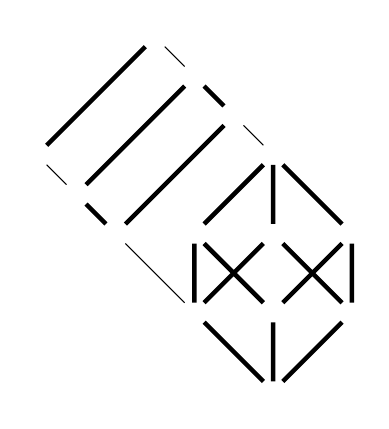
\begin{tikzpicture}
  \node(13) at (-1.5,1.5){};
  \node(12) at (-1,1){};
  \node(11) at (-3,0){};
  \node(10) at (-2.5,-0.5){};
  \node(9) at (-0.5, 0.5){};
  \node(8) at (-2, -1){};
  \draw[ultra thick] (13)--(11);
  \draw[ultra thick] (8)--(10)--(12)--(9);
  \draw(10)--(11)(12)--(13);
  \draw[ultra thick] (8)--(9);
  \node(7) at (0,0){};
  \node(6) at (0,-1){};
  \node(5) at (-1,-1){};
  \node(4) at (-1,-2){};
  \node(3) at (1,-1){};
  \node(2) at (1,-2){};
  \node(1) at (0,-2){};
  \node(0) at (0,-3){};
  \draw[ultra thick](4)--(5)--(7)--(6)--(4)
  (0)--(1)--(3)--(2)--(0)
  (0)--(4)(1)--(5)(2)--(6)(3)--(7);
  \draw(9)--(7) (8)--(4);
  \end{tikzpicture}
  \qquad
  \begin{tikzpicture}
  % \node at (0,-1)[n]{$M_{14,3}$};
  \node at (0,5)[n]{};
  \node(6) at (0,4){};
  \node(5) at (.5,2.5){};
  \node(4) at (-.5,2.5){};
  \node(3) at (1,1){};
  \node(2) at (-1,1){};
  \node(1) at (0,1){};
  \draw(4) edge (6);
  \draw(2) edge (4);
  \draw(1) edge (4);
  \draw (0,2.5) ellipse [x radius=25pt, y radius=13pt];
  \draw (0,1) ellipse [x radius=40pt, y radius=13pt];
  \end{tikzpicture}
  \caption{A fourteen-element ipo-semilattice with identity and its dual representation.}
  \label{m14,3}
\end{figure}

\begin{figure}[h!]
  \begin{center}
  \begin{tikzpicture}
  \node(13) at (-0.5,1.5){};
  \node(12) at (0,1){};
  \node(11) at (-1,1){};
  \node(10) at (-2.5,-0.5){};
  \draw[ultra thick] (13)--(12);
  \draw[ultra thick] (8)--(10)--(11)--(9);
  \draw(9)--(12)(11)--(13);
  \node(9) at (-0.5, 0.5){};
  \node(8) at (-2, -1){};
  \draw[ultra thick] (8)--(9);
  \node(7) at (0,0){};
  \node(6) at (0,-1){};
  \node(5) at (-1,-1){};
  \node(4) at (-1,-2){};
  \node(3) at (1,-1){};
  \node(2) at (1,-2){};
  \node(1) at (0,-2){};
  \node(0) at (0,-3){};
  \draw[ultra thick](4)--(5)--(7)--(6)--(4)
  (0)--(1)--(3)--(2)--(0)
  (0)--(4)(1)--(5)(2)--(6)(3)--(7);
  \draw(9)--(7) (8)--(4);
  \end{tikzpicture}
  \qquad
  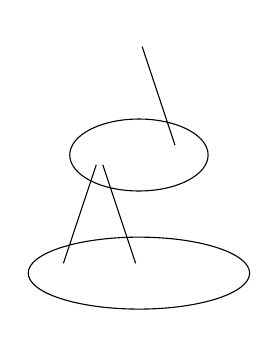
\begin{tikzpicture}
  % \node at (0,-1)[n]{$M_{14,4}$};
  \node(6) at (0,4){};
  \node(5) at (.5,2.5){};
  \node(4) at (-.5,2.5){};
  \node(3) at (1,1){};
  \node(2) at (-1,1){};
  \node(1) at (0,1){};
  \draw(5) edge (6);
  \draw(2) edge (4);
  \draw(1) edge (4);
  \draw (0,2.5) ellipse [x radius=25pt, y radius=13pt];
  \draw (0,1) ellipse [x radius=40pt, y radius=13pt];
  \end{tikzpicture}
  \end{center}
  \caption{Another fourteen-element ipo-semilattice with identity and its dual representation.}
  \label{m14,4}
\end{figure}

\begin{figure}[h!]
  \begin{center}
  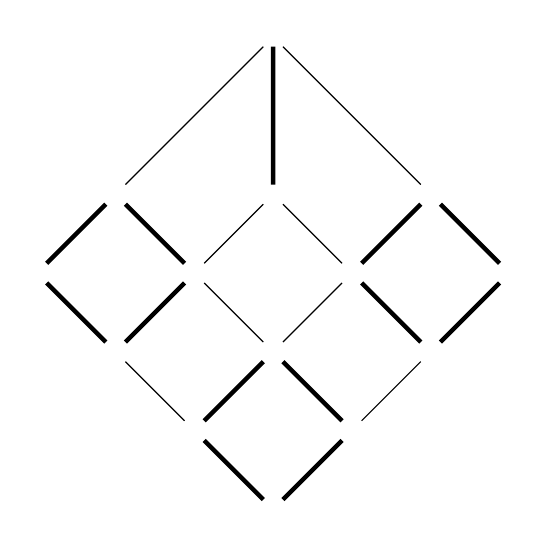
\begin{tikzpicture}
  \node(13) at (0, 3){};
  \node(12) at (0, 1){};
  \node(11) at (2,1){};
  \node(10) at (1, 0){};
  \node(9) at (3, 0){};
  \node(8) at (2,-1){};
  \node(7) at (-2,1){};
  \node(6) at (-3, 0){};
  \node(5) at (-1, 0){};
  \node(4) at (-2,-1){};
  \node(3) at (0,-1){};
  \node(2) at (-1, -2){};
  \node(1) at (1, -2){};
  \node(0) at (0,-3){};
  \draw[ultra thick] (2)--(3)--(1)--(0)--(2)(6)--(7)--(5)--(4)--(6)(10)--(11)--(9)--(8)--(10)(12)--(13);
  \draw(1)--(8)(3)--(10)(2)--(4)(3)--(5)(12)--(5)(12)--(10)(13)--(7)(13)--(11);
  \end{tikzpicture}
  \qquad
  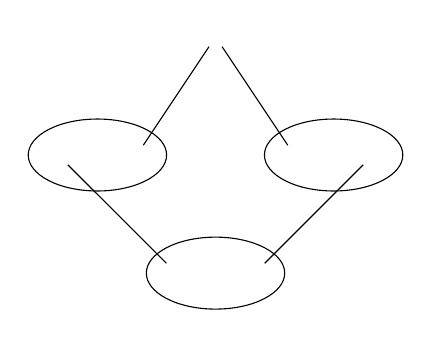
\begin{tikzpicture}
  % \node at (.5,-1)[n]{$M_{14,7}$};
  \node(7) at (.5,4){};
  \node(6) at (-1.5,2.5){};
  \node(5) at (-0.5,2.5){};
  \node(4) at (2.5,2.5){};
  \node(3) at (1.5,2.5){};
  \node(2) at (1,1){};
  \node(1) at (0,1){};
  \draw(5) edge (7);
  \draw(3) edge (7);
  \draw(2) edge (4);
  \draw(1) edge (6);
  \draw (0.5,1) ellipse [x radius=25pt, y radius=13pt];
  \draw (2,2.5) ellipse [x radius=25pt, y radius=13pt];
  \draw (-1,2.5) ellipse [x radius=25pt, y radius=13pt];
  \end{tikzpicture}
\end{center}
  \caption{Another fourteen-element ipo-semilattice with identity and its dual representation.}
  \label{m14,7}
\end{figure}

\begin{figure}[h!]
  \begin{center}
  
\begin{tikzpicture}
  \node(13) at (0, 3){};
  \node(12) at (-1, 2){};
  \node(11) at (2,1){};
  \node(10) at (1, 0){};
  \node(9) at (3, 0){};
  \node(8) at (2,-1){};
  \node(7) at (-2,1){};
  \node(6) at (-3, 0){};
  \node(5) at (-1, 0){};
  \node(4) at (-2,-1){};
  \node(3) at (0,-1){};
  \node(2) at (-1, -2){};
  \node(1) at (1, -2){};
  \node(0) at (0,-3){};
  \draw[ultra thick] (2)--(3)--(1)--(0)--(2)(6)--(7)--(5)--(4)--(6)(10)--(11)--(9)--(8)--(10)(12)--(13);
  \draw(1)--(8)(3)--(10)(2)--(4)(3)--(5)(12)--(10)(12)--(7)(13)--(11);
  \end{tikzpicture}
  \qquad
  \begin{tikzpicture}
  % \node at (.5,-1)[n]{$M_{14,8}$};
  \node(7) at (.5,4){};
  \node(6) at (-1.5,2.5){};
  \node(5) at (-0.5,2.5){};
  \node(4) at (2.5,2.5){};
  \node(3) at (1.5,2.5){};
  \node(2) at (1,1){};
  \node(1) at (0,1){};
  \draw[d](-.9,3) edge (7);
  \draw(3) edge (7);
  \draw(2) edge (4);
  \draw(1) edge (6);
  \draw (0.5,1) ellipse [x radius=25pt, y radius=13pt];
  \draw (2,2.5) ellipse [x radius=25pt, y radius=13pt];
  \draw (-1,2.5) ellipse [x radius=25pt, y radius=13pt];
  \end{tikzpicture}
\end{center}
  \caption{Another fourteen-element ipo-semilattice with identity and its dual representation.}
  \label{m14,8}
\end{figure}

\begin{figure}[h!]
  \begin{center}
  \begin{tikzpicture}
    \node(7) at (-1.5,1.5){};
    \node(6) at (-1.5,0.5){};
    \node(5) at (1.5,1.5){};
    \node(4) at (1.5,0.5){};
    \node(3) at (-1,1){};
    \node(2) at (0,2){};
    \node(1) at (1,1){};
    \node(0) at (0,0){};
    \draw (0)--(1)--(2)--(3)--(0);
    \draw (0)--(4)--(5)--(2);
    \draw (0)--(6)--(7)--(2);
\node at (0,-1)[n]{$\leq$};
  \end{tikzpicture}
  \qquad \qquad
  \begin{tikzpicture}
    \node(7) at (-1,4){};
    \node(6) at (-1,3){};
    \node(5) at (1,4){};
    \node(4) at (1,3){};
    \node(3) at (-1,1){};
    \node(2) at (0,2){};
    \node(1) at (1,1){};
    \node(0) at (0,0){};
    \draw[ultra thick] (0)--(1)--(2)--(3)--(0);
    \draw (2)--(4);
    \draw (2)--(6);
    \draw[ultra thick] (4)--(5);
    \draw[ultra thick] (6)--(7);
\node at (0,-1)[n]{$\sqsubseteq$};
  \end{tikzpicture}
\end{center}
  \caption{An 8-element i$\ell$-semilattice. Its multiplicative order shows its unital sub-i$\ell$-semilattices.}
  \label{subsemilattice}
\end{figure}
\clearpage
\begin{thebibliography}{9}
\bibitem{BLP2019}
Bonzio, S., Loi, A., Peruzzi, L.: A duality for involutive bisemilattices, Studia Logica, (2019) 107: 423--444.

\bibitem{GJKO2007}
Galatos, N., Jipsen, P., Kowalski, T., Ono, H.: ``Residuated
lattices: an algebraic glimpse at substructural logics'', Studies
in Logic and the Foundations of Mathematics, Vol. 151, Elsevier, 2007.


\bibitem{JTV2020}
Jipsen, P., Tuyt, O., Valota, D.: Structural characterization of commutative idempotent involutive residuated lattices, preprint, 2020.

\bibitem{McC2010}
McCune, W.: Prover9 and Mace4. \url{www.cs.unm.edu/~mccune/prover9/}, 2005–2010.
\end{thebibliography}
\end{document}
